\documentclass[10pt,aspectratio=169]{beamer}

% All the boilerplate is in deslides.sty
\usepackage{deslides}

\author{Ji\v{r}\'i Lebl}

\institute[OSU]{%
Oklahoma State University%
%Departemento pri Matematiko de Oklahoma {\^S}tata Universitato%
}

\title{28. Dirac delta and impulse response (Laplace transform)\\(Notes on Diffy Qs, 6.4)}

\date{}

\begin{document}

\begin{frame}
\titlepage

%\bigskip

\begin{center}
The textbook: \url{https://www.jirka.org/diffyqs/}

or \url{https://jirilebl.github.io/diffyqs/}
\end{center}
\end{frame}

\begin{frame}
A way to study a physical system is by putting

in a short pulse and seeing the output.

\medskip
\pause

Simplest is a \emph{rectangular pulse}:

\medskip

$
\qquad
\displaystyle
\varphi(t) = 
\begin{cases}
0 & \text{if } \; \phantom{a \leq {}} t < a , \\
M & \text{if } \; a \leq t < b , \\
0 & \text{if } \; b \leq t .
\end{cases}
$

\vspace*{-1.0in}

\hspace*{2.8in}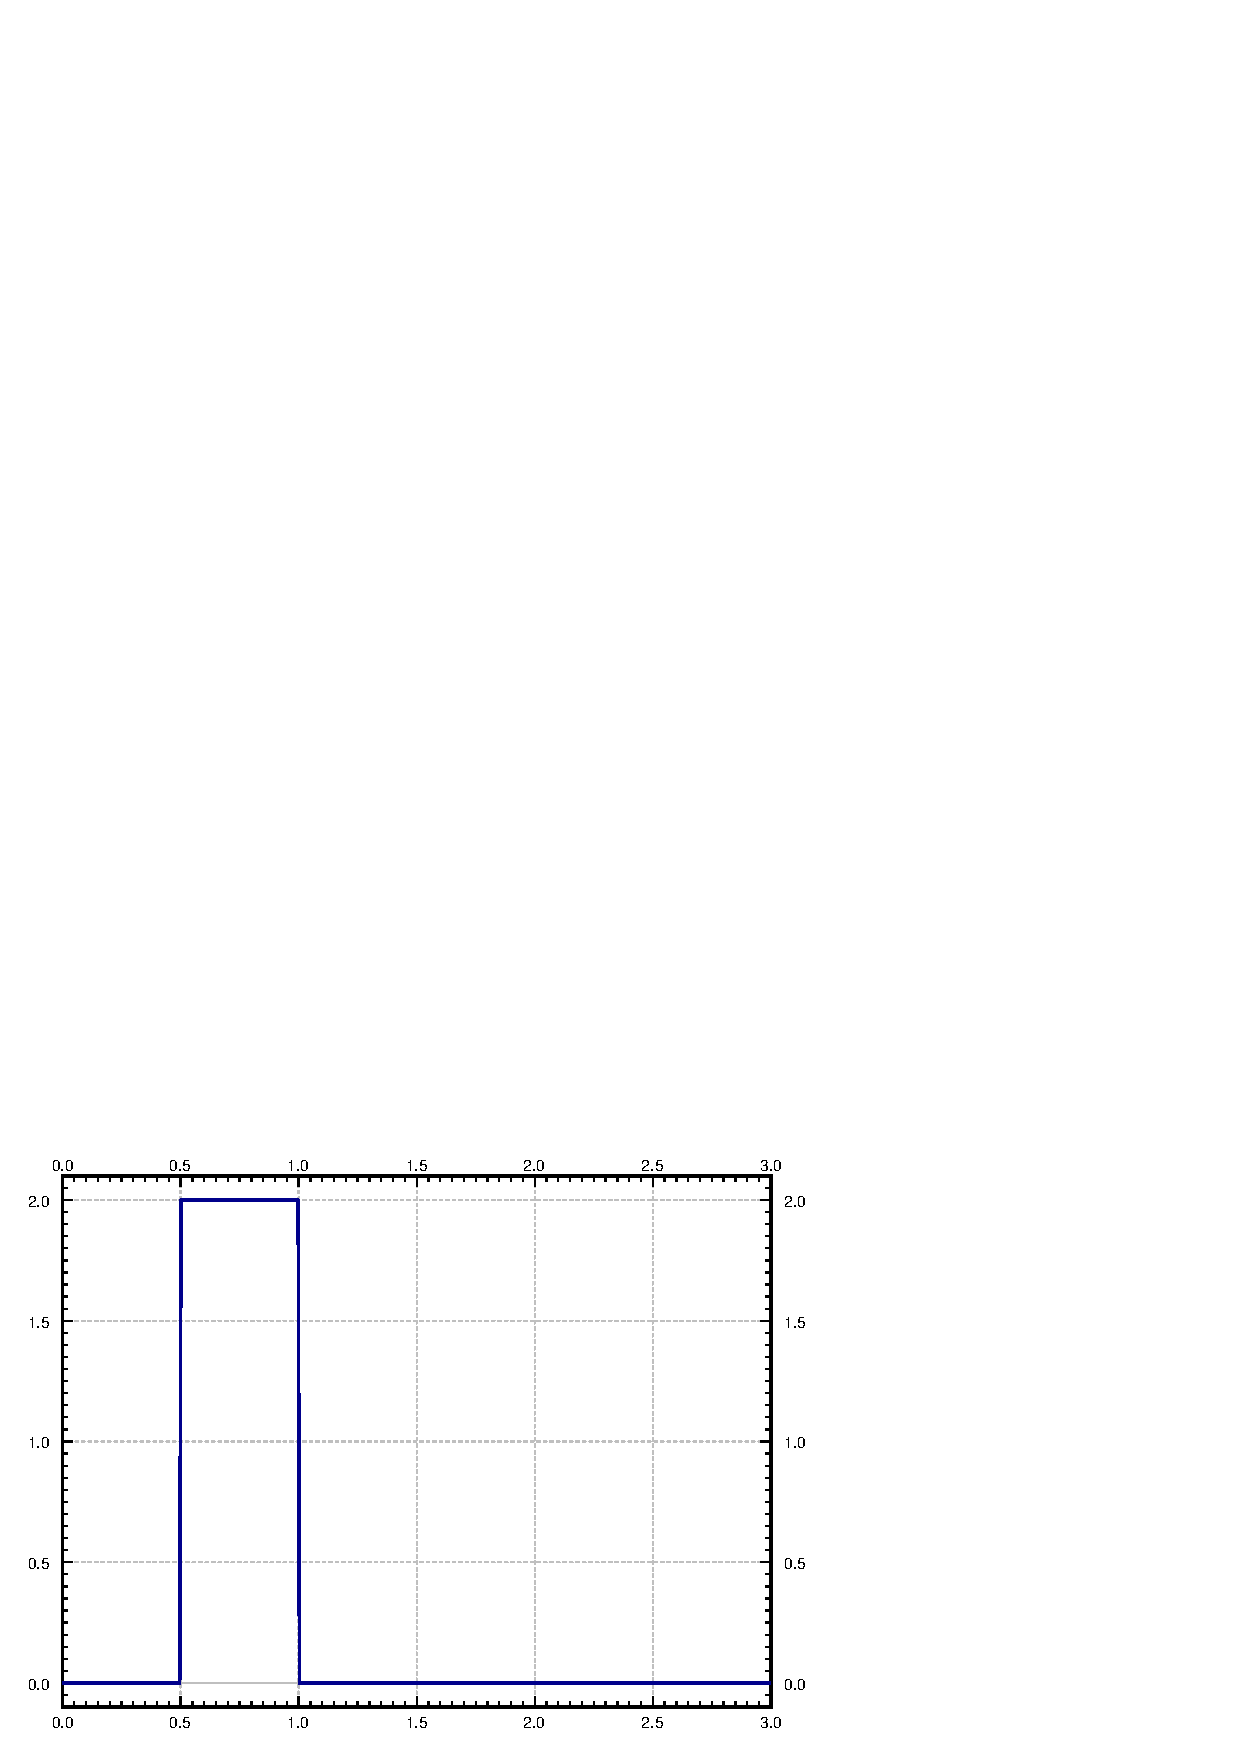
\includegraphics[width=2.8in]{../figures/lt-sqpulse}

\hspace*{2.8in}
\quad
Rectangular pulse $a=0.5$, $b=1$, $M = 2$.

\vspace*{-1.2in}
\pause

Notice: \quad
$\varphi(t) = M \bigl( u(t-a) - u(t-b) \bigr)$.

($u(t)$ is the unit step function.)

\medskip
\pause

The Laplace transform is

\medskip

$\qquad \displaystyle
\begin{aligned}
{\mathcal{L}} \bigl\{ \varphi(t) \bigr\}
& =
{\mathcal{L}} \bigl\{ M \bigl( u(t-a) - u(t-b) \bigr)  \bigr\}
\\
\pause
& =
M
\frac{e^{-as} - e^{-bs}}{s} .
\end{aligned}
$

\medskip
\pause

Let $a=0$ and $M=\nicefrac{1}{b}$ so that
$\int_0^\infty \varphi(t) \,dt = 1$.
\pause
\quad
$\varphi(t) = \frac{u(t) - u(t-b)}{b}$
is
a pulse of ``unit mass''.
\end{frame}

\begin{frame}
For this unit mass pulse we get
\[
{\mathcal{L}} \bigl\{ \varphi(t) \bigr\}
=
{\mathcal{L}} \left\{ \frac{u(t) - u(t-b)}{b}  \right\}
=
\frac{1 - e^{-bs}}{bs} .
\]
\pause
Letting $b \to 0$, we obtain the \emph{Dirac delta function}
$\delta(t)$.

\medskip
\pause

Note that
\quad
$\displaystyle
\lim_{b \to 0}
\frac{1-e^{-bs}}{bs} = 1$
\quad
so \quad ${\mathcal{L}} \bigl\{ \delta(t) \bigr\} = 1$.

\medskip
\pause

There is no such ``function'' (it is a ``generalized function'')

\medskip
\pause

It is a ``function'' where
for any continuous $f(t)$,
\[
\int_{-\infty}^\infty \delta(t) f(t) \,dt = f(0) .
\]
\pause
For an interval
\[
\int_c^d \delta(t) \,dt = 
\begin{cases}
1 & \text{if the interval $[c,d]$ contains 0, i.e.\ } c \leq 0 \leq d, \\
0 & \text{otherwise.}
\end{cases}
\]
(We think of $\int_c^d$ really as $\int_{c-}^{d+}$)

\end{frame}

\begin{frame}

$\delta(t)$ is a ``function'' with all the ``mass'' at $t=0$.

\medskip
\pause

Informally $\delta(t)$ is zero for $t \neq 0$ and very infinite at $t=0$.

\medskip
\pause

It is a ``limit'' of pulses of decreasing length
of integral $1$ such as
\quad
$\varphi(t) = \dfrac{u(t) - u(t-b)}{b}$.

\medskip
\pause

For small $b$ and continuous $f(t)$,
\[
\int_{-\infty}^\infty \varphi(t) f(t) \,dt =
\int_{-\infty}^\infty \frac{u(t) - u(t-b)}{b} f(t) \,dt
\pause
=
\frac{1}{b} \int_{0}^b f(t) \,dt
\pause
\approx
\frac{1}{b} \int_{0}^b f(0) \,dt = f(0) .
\]

\pause
$\delta(t)$ is taking limit as $b \to 0$.

\medskip
\pause

It is not a function, but it is something we can integrate.

\medskip
\pause

We often shift by $a$ as $\delta(t-a)$.  Then:
\qquad
$\displaystyle
\int_{-\infty}^\infty \delta(t-a) f(t) \,dt = f(a) .
$

\medskip
\pause

Note that $\delta(a-t)$ is the same as $\delta(t-a)$.

So the convolution of $\delta(t)$ with $f(t)$ is again $f(t)$:
\qquad
$\displaystyle
(f * \delta) (t) = 
\int_{0}^t f(\tau) \delta(t-\tau) \,d\tau
= f(t) .
$
\end{frame}

\begin{frame}
Compute the Laplace transform:
\[
{\mathcal{L}} \bigl\{ \delta(t-a) \bigr\}
=
\int_{0}^\infty e^{-st} \delta(t-a) \,dt = e^{-as} .
\qquad
\text{In particular,}
\qquad
{\mathcal{L}} \bigl\{ \delta(t) \bigr\} = 1 .
\]
\medskip
\pause

\textbf{Example:}
Find ${\mathcal{L}}^{-1} \left\{ \frac{s+1}{s} \right\}$.
Note that $\frac{s+1}{s}$ is not a proper rational function.
\pause
\[
{\mathcal{L}}^{-1} \left\{ \frac{s+1}{s} \right\}
=
{\mathcal{L}}^{-1} \left\{ 1 + \frac{1}{s} \right\}
\pause
=
{\mathcal{L}}^{-1} \{ 1 \}
+
{\mathcal{L}}^{-1} \left\{ \frac{1}{s} \right\}
\pause
=
\delta(t) + 1 .
\]

\pause
\medskip

\emph{Remark:}
$
{\mathcal{L}} \bigl\{ u(t-a) \bigr\} = \frac{e^{-as}}{s}
$.

\pause
If $u(t-a)$ had a derivative,
its Laplace transform would be
$s \frac{e^{-as}}{s} = e^{-as}$.
\pause
Moreover
\[
\int_0^t \delta(s-a)\,ds = u(t-a) .
\]
\pause
So in some sense
\[
\text{``}
\quad \frac{d}{dt} \Bigl[ u(t-a) \Bigr] = \delta(t-a) . \quad
\text{''}
\]
\end{frame}

\begin{frame}
For a differential equation $L x = f(t)$,
think of $f(t)$ as the input, and $x(t)$ as the output.

\medskip
\pause

The solution to
\[
L x = \delta(t)
\]
is called the \emph{impulse response}.

\pause
\medskip

\textbf{Example:}
Solve (find the impulse response)
\[
x'' + \omega_0^2 x = \delta(t) , \quad x(0) = 0, \quad x'(0) = 0 .
\]

\pause
Apply the Laplace transform as usual:
\[
s^2 X(s) + \omega_0^2 X(s) = 1 ,
\qquad \text{and so} \qquad
X(s) = \frac{1}{s^2+ \omega_0^2} .
\]
\pause
Inverse Laplace transform gives
\[
x(t) = 
\frac{\sin (\omega_0 t)}{\omega_0} \qquad \text{for } t > 0 .
\]

\pause
\emph{Remark:}
Is $x'(0)=0$?
\pause
Think $x(t)=0$ for $t \leq 0$.
Then $x(t)$
has a ``corner'' at $t=0$,
$x'$ has a jump discontinuity,
and $x''$ produces the $\delta(t)$.
\pause
Really we have $x'(0-) = \lim_{t \uparrow 0} x'(0) = 0$.

\end{frame}

\begin{frame}
Solution to $x'' + \omega_0^2 x = f(t)$ is
\[
x(t) = 
\int_0^t
f(\tau) 
\frac{\sin \bigl( \omega_0 (t-\tau) \bigr)}{\omega_0} \, d\tau .
\]
That is, \emph{the solution for an arbitrary input is given as
convolution with the impulse response}.

\medskip
\pause

Why? \pause  Suppose $f(t)$ and $h(t)$ are zero for $t < 0$,
\[
(f * h)''(t) =
\frac{d^2}{dt^2}\left[
\int_0^t
f(\tau) 
h(t-\tau) \, d\tau \right]
\pause
=
\int_0^t
f(\tau) 
h''(t-\tau) \, d\tau
\pause
= (f * h'')(t) .
\]
\pause
If $h(t)$ is the impulse response, then
\[
f * (h'' + \omega_0^2 h) =
\pause
(f * h'') + \omega_0^2 (f * h) =
(f * h)'' + \omega_0^2 (f * h) .
\]
\pause
and
\[
(f * \delta)(t) = f(t).
\]
\pause
So 
$x(t) = (f * h)(t)$ is the solution to
$x'' + \omega_0^2 x = f(t)$.

\medskip
\pause

Same procedure works for any constant-coefficient linear equation $Lx = f(t)$.

\medskip
\pause

Note that
$h(t) = {\mathcal{L}}^{-1} \bigl\{ H(s) \bigr\}$
where $H(s)$ is the transfer function.

\end{frame}

\begin{frame}
Consider a different application of $\delta$ functions:
Representing point loads on a beam.

\pause
\medskip

A steel beam has length $L$, supported simply at the ends.

$x$ is the position.  $y(x)$ is the deflection at $x$.
%
A point load of force $F$ down is at $x=a$.

\begin{center}
\scalebox{0.9}{\subimport*{../figures}{beam-bending.pdf_t}}
\end{center}
\pause

$y$ satisfies the
\emph{Euler--Bernoulli equation}:
\qquad
$EI \dfrac{d^4 y}{dx^4} = F(x)$.
\quad ($E,I$ constants, $F(x)$ force at $x$)

\pause
\medskip

For a point load as above:
\[
EI \frac{d^4 y}{dx^4} = -F \delta(x-a) .
\]
\pause
\medskip
The end points satisfy:
\[
y(0) = 0, \qquad y''(0) = 0, \qquad
y(L) = 0, \qquad y''(L) = 0.
\]
\end{frame}

\begin{frame}

\textbf{Example:}
Suppose length is 2, $EI=1$, $F=1$ and $a=1$:
\[
\frac{d^4 y}{dx^4} = -\delta(x-1) ,
\qquad
y(0) = 0, \quad y''(0) = 0, \quad
y(L) = 0, \quad y''(L) = 0.
\]
\pause
We apply Laplace in $x$ rather than $t$.
Write $Y(s)$ for $\mathcal{L} \{ y(x) \}$.
\[
s^4Y(s)-s^3y(0)-s^2y'(0)-sy''(0)-y'''(0)
= -e^{-s}.
\]
\pause
We have $y(0) = 0$ and $y''(0) = 0$.  We call $C_1 = y'(0)$ and $C_2=y'''(0)$.
\pause
Solve:
\[
Y(s) = \frac{-e^{-s}}{s^4} + \frac{C_1}{s^2}+ \frac{C_2}{s^4} .
\]
\pause
We take the inverse (using the second shifting property)
\[
y(x) = \frac{-{(x-1)}^3}{6} u(x-1) + C_1 x + \frac{C_2}{6} x^3 .
\]
\end{frame}

\begin{frame}
\[
y(x) = \frac{-{(x-1)}^3}{6} u(x-1) + C_1 x + \frac{C_2}{6} x^3 .
\]
We still need to apply $y(2) = 0$ and $y''(2) = 0$.
\pause
\[
0 = y(2) = \frac{-{(2-1)}^3}{6} + C_1 (2) + \frac{C_2}{6} 2^3
\pause
=
\frac{-1}{6} + 2 C_1 + \frac{4}{3} C_2 ,
\]
\pause
Note that for $x$ near 2, $u(x-1)=1$ so
\[
0 = y''(2) = \frac{-3\cdot 2 \cdot (2-1)}{6} + \frac{C_2}{6} 3\cdot 2 \cdot 2
\pause
 = -1 + 2 C_2 .
\]
\pause
We get $C_2 = \frac{1}{2}$ and $C_1 = \frac{-1}{4}$.
\pause
Hence,
\[
y(x) = \frac{-{(x-1)}^3}{6} u(x-1) - \frac{x}{4} + \frac{x^3}{12} .
\]
\end{frame}

\end{document}
